\begin{figure}[t]
\centering
\subfloat[Latent space temporal interpolation module.]{%
    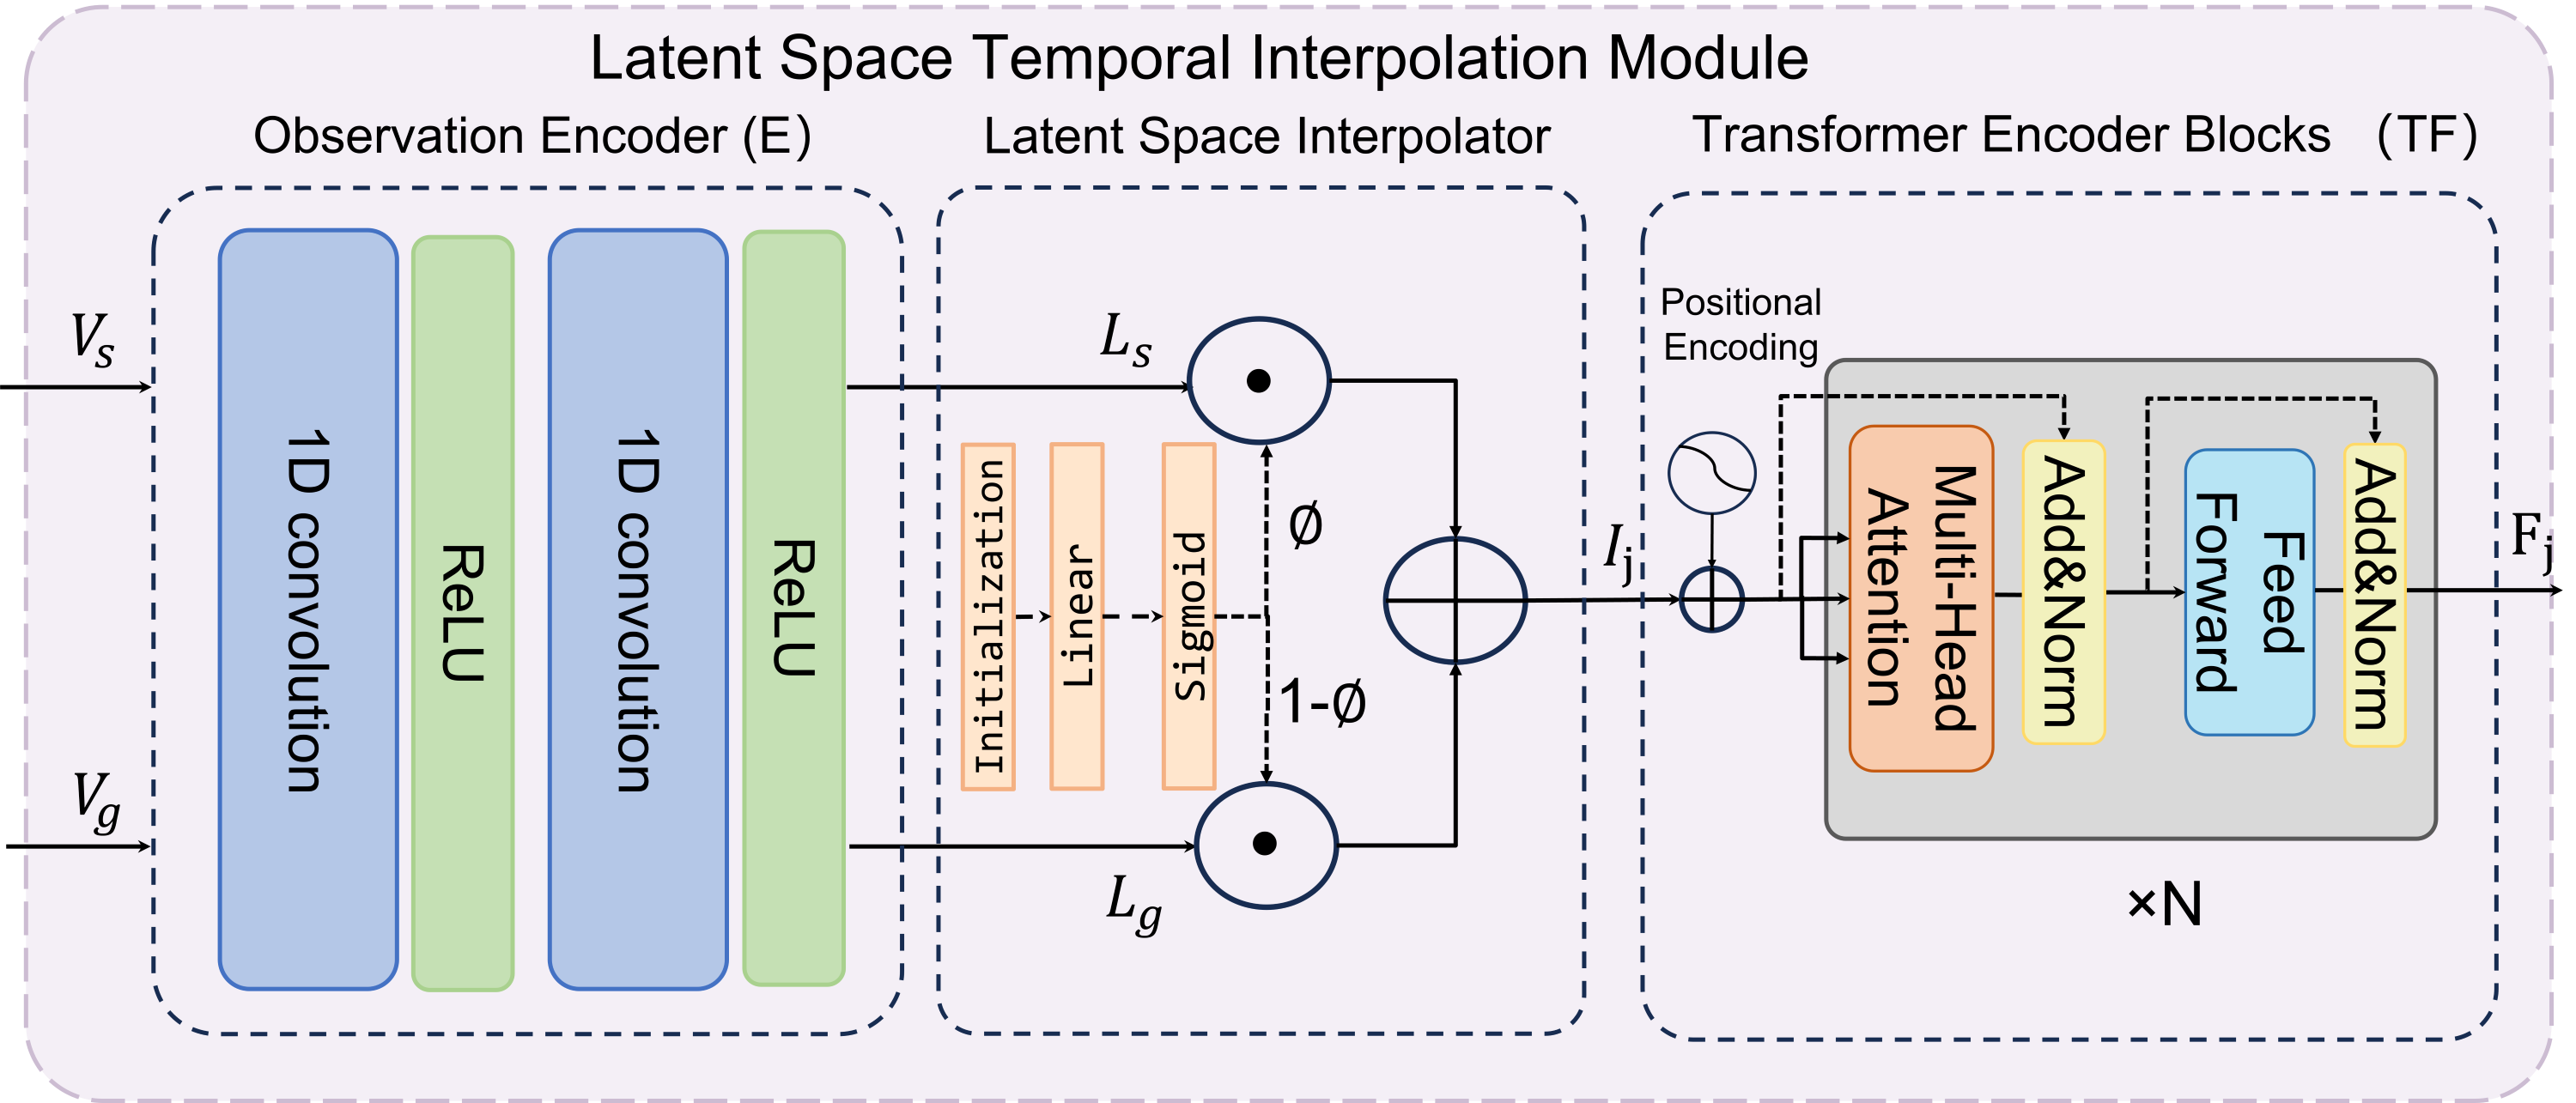
\includegraphics[width=0.48\textwidth, height=0.135\textheight]{figures/architecture2.png}
    \label{fig:architecture2}
}
\hspace{0.1cm} 
\subfloat[Residual temporal block \& cross-attention module.]{%
    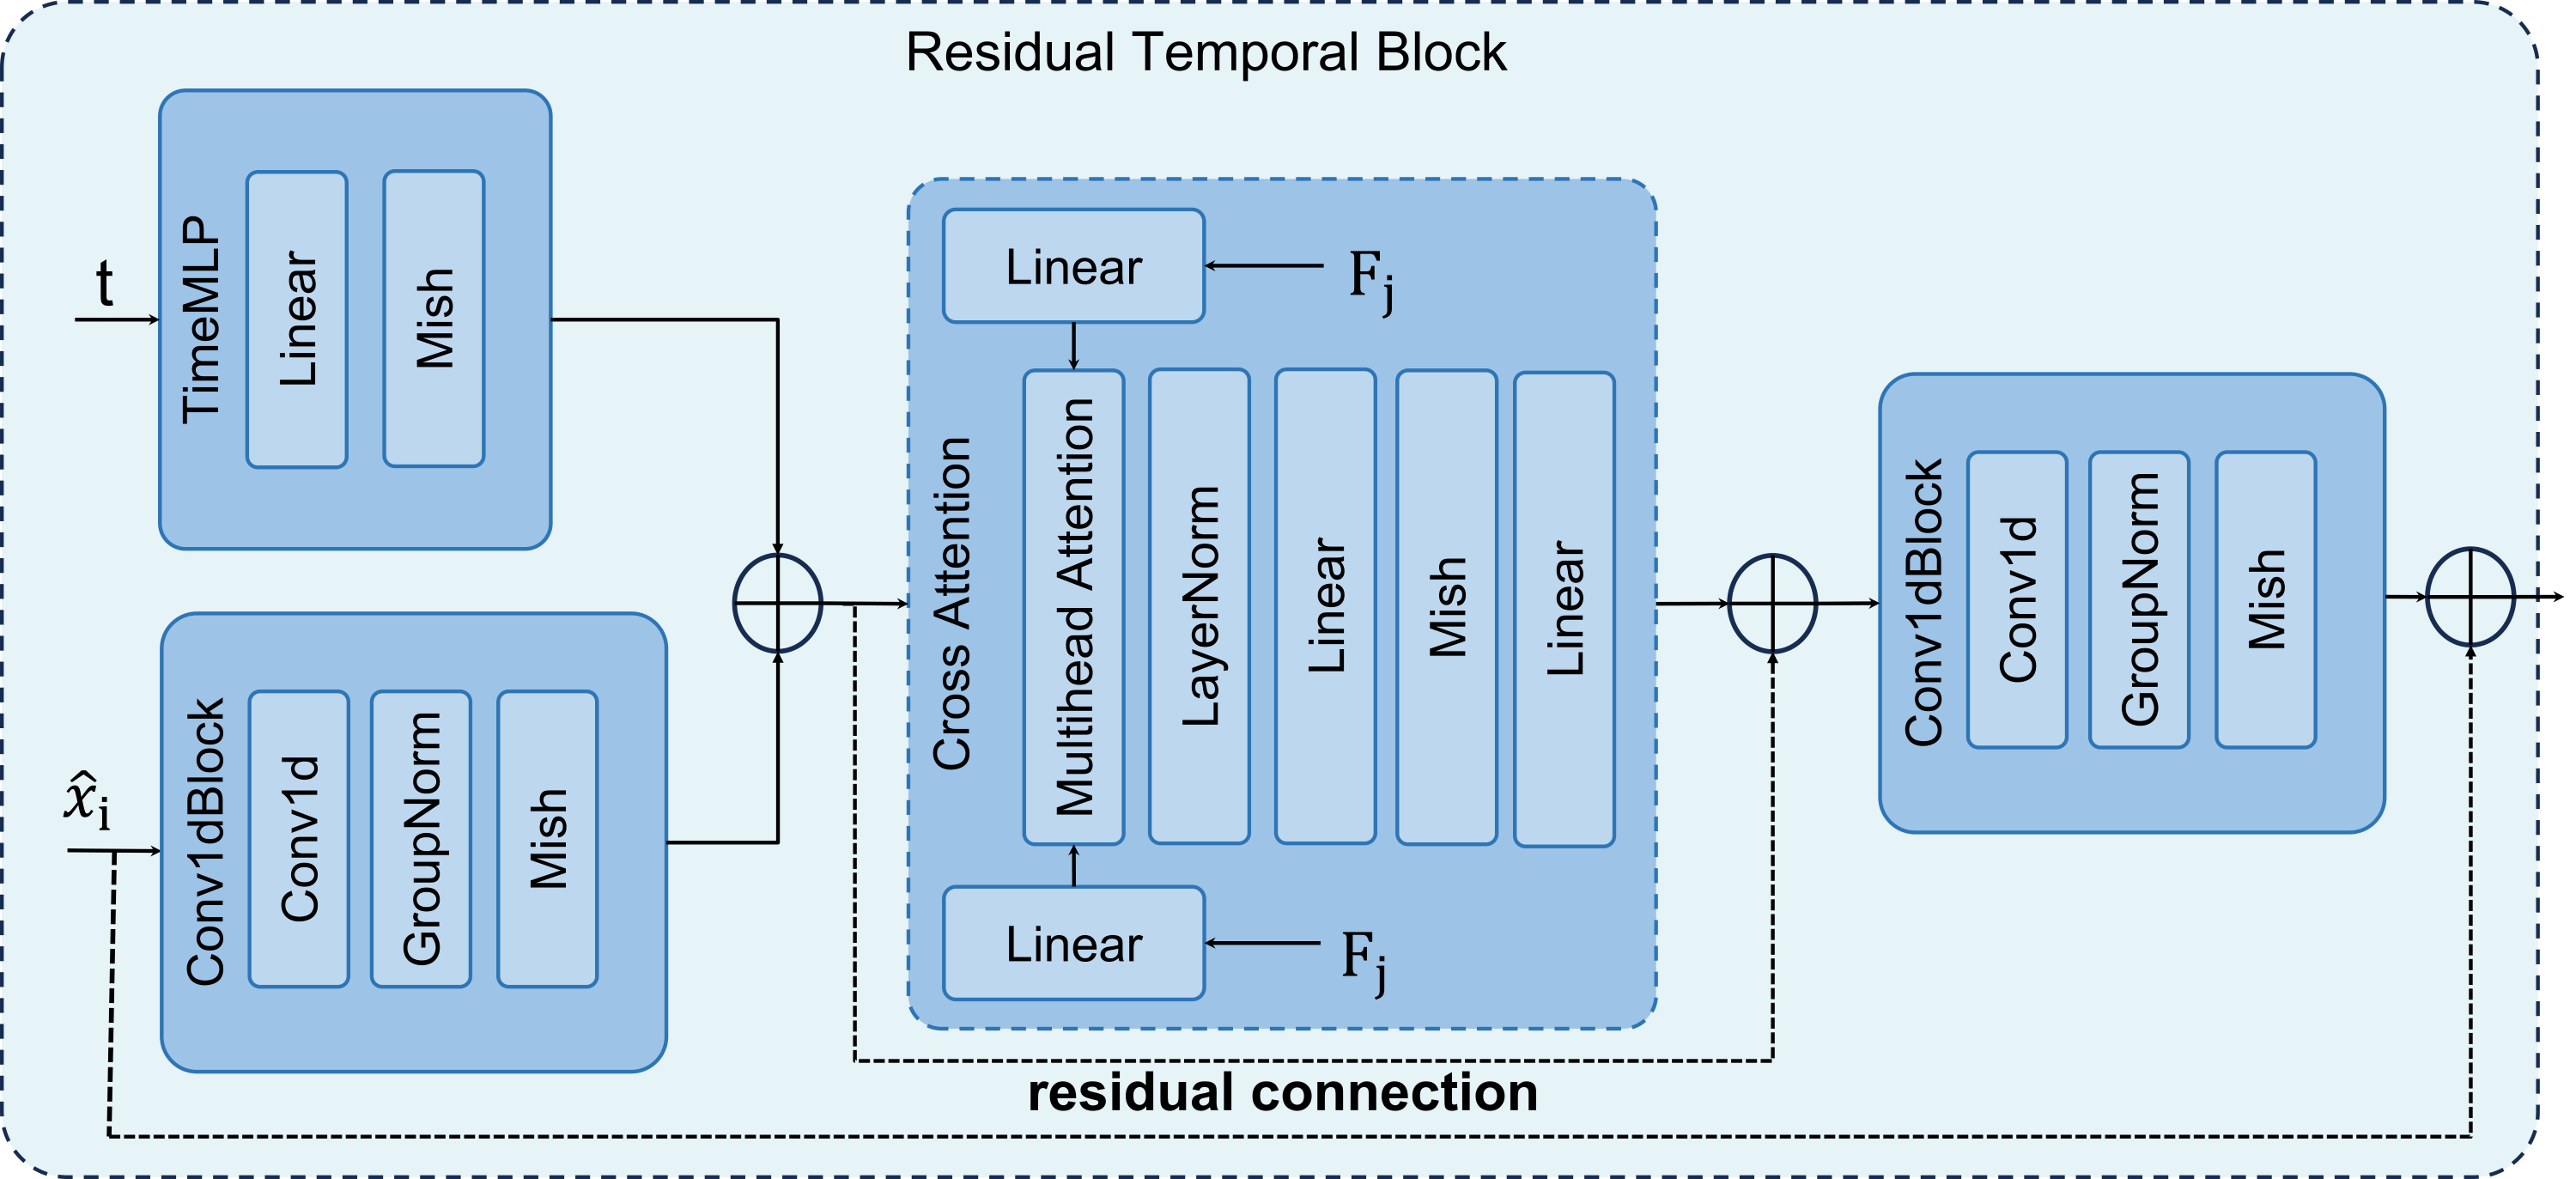
\includegraphics[width=0.48\textwidth, keepaspectratio]{figures/architecture3.png}
    \label{fig:architecture3}
}
\caption{ \textcolor{orange}{Module in \Cref{fig:architecture2} generates temporally coherent latent features from observations, while the block in \Cref{fig:architecture3} refines these features with temporal dependencies, guiding coherent action sequence generation.} }
\label{fig:architecturek}
\vspace{-3mm}
\end{figure}